\documentclass[a4paper]{article}

\usepackage{a4wide}
\usepackage{amsmath}
\usepackage{amssymb}
\usepackage{amsthm}
\usepackage{enumitem}
    \setlist[enumerate]{label=(\alph*),itemsep=3pt,topsep=6pt}
    \setlist[itemize]{itemsep=3pt,topsep=6pt}
\usepackage{tikz}
\usepackage[utf8]{inputenc}

\theoremstyle{plain}
\newtheorem*{theorem*}{Věta}
\theoremstyle{definition}
\newtheorem{problem}{Příklad}
\newtheorem*{ukol}{Domácí úkol}


\begin{document}

\section*{NAIL062 V\&P Logika: 6. cvičení}


\textbf{Témata:} 
Rezoluce ve výrokové logice. Aplikace věty o kompaktnosti. Hilbertův kalkulus.


\medskip\begin{problem}
Označme jako $\varphi$ výrok $\neg (p \vee q) \to (\neg p \wedge \neg q)$. Ukažte, že $\varphi$ je tautologie:
\begin{enumerate}
    \item Převeďte $\neg \varphi$ do CNF a zapište výsledný výrok jako formuli $S$ v množinové reprezentaci.
    \item Najděte rezoluční zamítnutí $S$.
\end{enumerate}
\end{problem}


\medskip\begin{problem}
Najděte rezoluční zamítnutí následujících výroků:
\begin{enumerate}
    \item $(p\leftrightarrow (q\to r))\wedge((p\leftrightarrow q)\wedge(p\leftrightarrow \neg r))$
    \item $\neg(((p\to q)\to \neg q)\to \neg q)$
\end{enumerate}
\end{problem}
    
    
\medskip\begin{problem}
Dokažte rezolucí, že v teorii $T=\{\neg p \to \neg q,\neg q \to \neg r, (r\to p)\to s\}$ platí výrok $s$.
\end{problem}


\medskip\begin{problem}Nechť prvovýroky $r$, $s$, $t$  reprezentují (po řadě), že \emph{``Radka / Sára / Tom je ve škole''} a označme $\mathbb{P}=\{r,s,t\}$. Víme, že
    \begin{itemize}\it
    \item Není-li Tom ve škole, není tam ani Sára.
    \item Radka bez Sáry do školy nechodí.
    \item Není-li Radka ve škole, je tam Tom.
    \end{itemize}
    \begin{enumerate}
    \item Formalizujte naše znalosti jako teorii $T$ v jazyce $\mathbb P$.
    \item Rezoluční metodou dokažte, že z $T$ vyplývá, že \emph{Tom je ve škole}: Napište formuli $S$ v množinové reprezentaci, která je nesplnitelná, právě když to platí, a najděte rezoluční zamítnutí $S$. Nakreslete rezoluční strom.
    \item Určete množinu modelů teorie $T$.
    \end{enumerate}
\end{problem}


\medskip\begin{problem}
\emph{Half-adder circuit} je logický obvod se dvěma vstupními bity (bit 1, bit 2) a dvěma výstupními bity (carry, sum) znázorněný v následujícím diagramu:
\begin{center}
    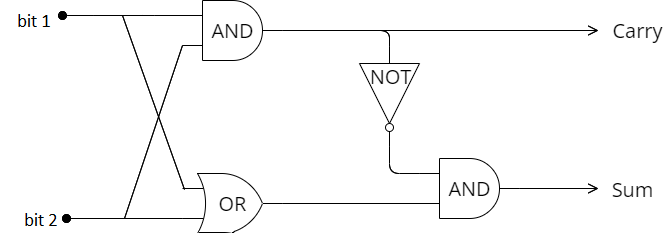
\includegraphics[width=0.5\textwidth]{files/half-adder.png}
\end{center}
\begin{enumerate}
        \item Formalizujte tento obvod ve výrokové logice. Konktrétně, vyjádřete jej jako výrokovou teorii $T=\{c\leftrightarrow \varphi,\ s\leftrightarrow \psi\}$ v jazyce $\mathbb P=\{b_1,b_2,c,s\}$, kde výrokové proměnné znamenají po řadě ``bit 1'', ``bit 2'', ``carry'' a ``sum'', a formule $\varphi,\psi$ neobsahují proměnné $c,s$.
        %\item Axiomatizujte teorii $T$ výrokem v CNF a také výrokem v DNF
        \item Dokažte rezoluční metodou, že $T\models c\to\neg s$.
\end{enumerate}
\end{problem}


\medskip\begin{problem} Máme k dispozici MgO, H$_2$, O$_2$, a C, a můžeme provádět následující reakce:
    \begin{itemize}
        \item MgO\ +\ H$_2$\ \ $\to$\ \ Mg\ +\ H$_2$O
        \item C\ +\ O$_2$\ \ $\to$\ \ CO$_2$
        \item CO$_2$\ +\ H$_2$O\ \ $\to$\ \ H$_2$CO$_3$
    \end{itemize}
    \begin{enumerate}
        \item Reprezentujte naše možnosti výrokem (nad vhodně zvoleným jazykem) a převeďte ho do množinové reprezentace.
        \item Pomocí rezoluce dokažte, že můžeme získat H$_2$CO$_3$. Lze najít LI-důkaz téhož?
    \end{enumerate}
\end{problem}


\medskip\begin{problem}
Celá čísla postihla záhadná nemoc šířící se (v diskrétních krocích) dle následujících pravidel (platících pro všechna čísla ve všech krocích).
\begin{enumerate}[label=(\roman*)]\it
\item Zdravé číslo onemocní, právě když je právě jedno číslo nemocné (v předchozím čase).
\item Nemocné číslo se uzdraví, právě když je předchozí číslo nemocné (v předchozím čase).
\item V čase $0$ bylo nemocné číslo $0$, ostatní čísla byla zdravá.
\end{enumerate}
%(Sousedními čísly čísla $i$ myslíme $i-1$ a $i+1$, předchozím číslem myslíme $i-1$.)
\begin{enumerate}
\item Napište teorie $T_1, T_2, T_3$ vyjadřující (po řadě) tvrzení $(i), (ii), (iii)$ nad množinou prvovýroků $\mathbb{P}=\{p_i^t \mid i\in\mathbb{Z}, t\in\mathbb{N}_0\}$, kde prvovýrok $p_i^t$ vyjadřuje, že ``{\it číslo $i$ je v čase $t$ nemocné.}''
\item Převeďte axiomy z $T_1, T_2, T_3$ do CNF a napište teorii $S$ v množinové reprezentaci, která je nesplnitelná, právě když $T_1 \cup T_2 \cup T_3 \models \neg p_1^2$, tj.: ``{\it Číslo $1$ je zdravé v čase $2$.}'' (Stačí převést jen konkrétní axiomy z $T_1,T_2,T_3$, ze kterých plyne $\neg p_1^2$, a do $S$ uvést jen příslušné klauzule.)
\item Rezolucí dokažte, že $S$ je nesplnitelná. Zamítnutí znázorněte rezolučním stromem.
\end{enumerate}
\end{problem}


\medskip\begin{problem}
    Najděte rezoluční uzávěry $\mathcal{R}(S)$ pro následující výroky $S$:
    \begin{enumerate}
        \item $\{\{p,q\},\{p,\neg q\},\{\neg p,\neg q\}\}$
        \item $\{\{p,\neg q,r\},\{q,r\},\{\neg p, r\},\{q,\neg r\},\{\neg q\}\}$
    \end{enumerate}
\end{problem}
    
    
\medskip\begin{problem}
    Zkonstruujte \emph{strom dosazení} pro formuli $S=\{\{p,r\},\{q,\neg r\},\{\neg q\},\{\neg p,t\},\{\neg s\},\{s,\neg t\}\}$.
\end{problem}


\medskip\begin{problem}
    Dokažte podrobně, že je-li $S=\{C_1,C_2\}$ splnitelná a $C$ je rezolventa $C_1$ a $C_2$, potom je i $C$ splnitelná.
\end{problem}

    
\medskip\begin{problem} Dokažte pomocí věty o kompaktnosti a variant tvrzení pro konečné objekty:
\begin{enumerate}
    \item Každý spočetný rovinný graf je obarvitelný čtyřmi barvami.
    \item Každé spočetné částečné uspořádání lze rozšířit na úplné (lineární) uspořádání.
    %\item Hallova věta platí i pro nekonečné množiny.
\end{enumerate}

\end{problem}



\medskip\begin{problem}
V Hilbertově kalkulu dokažte pro libovolné formule následující vztahy:
\begin{enumerate}
    %\item $\vdash_H\ p\to p$
    \item $\{\neg p\}\ \vdash_H\ p\to q$
    \item $\{\neg(\neg p)\}\ \vdash_H\ p$
    \item $\{p\to q,q \to r\}\ \vdash_H\ p\to r$
\end{enumerate}    
\end{problem}

\medskip\begin{problem}
    Dokažte korektnost Hilbertova kalkulu:
    \begin{itemize}
        \item Dokažte, že logické axiomy jsou tautologie.
        \item Dokažte, že modus ponens je korektní, tj. když $T\models\varphi$ a $T\models\varphi\to\psi$, tak $T\models\psi$.
        \item Ukažte, že $T\ \vdash_H\ \varphi$ implikuje $T\models\varphi$.
    \end{itemize}
    \end{problem}
    
\medskip\begin{problem}
    Vyslovte a dokažte větu o dedukci pro Hilbertův kalkul.
\end{problem}
    


\medskip\begin{ukol}
Tentokrát žádný není. Místo domácího úkolu se připravte na zápočtový test: procvičte rezoluční metodu a vyřešte vzorový test (na webu).
\end{ukol}

\end{document}